\documentclass[10pt,sigconf,letterpaper,anonymous]{acmart}

\usepackage[english]{babel}
\usepackage{balance}
  % for creating a balanced last page (usually last page with references)

\usepackage{booktabs} % For formal tables
\usepackage{pifont}
\usepackage{color}
\usepackage{adjustbox}
% \usepackage[dvipsnames]{xcolor}
\usepackage{microtype} % must be loaded after all fonts
% \usepackage{url}
\usepackage{makecell}
\usepackage{graphicx, subfigure}
% \usepackage{subcaption}
\usepackage{amsmath}

\usepackage[shortlabels]{enumitem}

\usepackage{multirow}
\usepackage{booktabs}
% Used in Appendix tables
\usepackage{makecell}
\renewcommand\cellalign{cl}
\renewcommand\cellgape{\Gape[1pt]}

\def\BibTeX{{\rm B\kern-.05em{\sc i\kern-.025em b}\kern-.08emT\kern-.1667em\lower.7ex\hbox{E}\kern-.125emX}}

\renewcommand\footnotetextcopyrightpermission[1]{} % removes footnote with conference information in first column
\pagestyle{plain} % removes running headers
\settopmatter{printacmref=false}
\setcopyright{none}


% %Conference Info
% \acmYear{2018}
% \copyrightyear{2018}
% \setcopyright{acmcopyright}
% \acmConference{CoNEXT '18}{December 4--7, 2018}{Heraklion/Crete, Greece}
% \acmPrice{TBA}
% \acmDOI{TBA}
% \acmISBN{TBA}

\providecommand{\myparab}[1]{\smallskip\noindent\textbf{#1} }
\newcommand{\sectionref}[1]{$\S$\ref{#1}}
\newcommand{\phong}[1]{\ding{110}\ding{43}\textcolor{blue}{NP: #1}}
\newcommand{\arjun}[1]{\textcolor{green}{ANB: #1}}
\newcommand{\todo}[1]{\textcolor{red}{To-do: #1}}
\newcommand{\chase}[1]{\textcolor{purple}{CJ: #1}}
\newcommand{\eg}{\textit{e.g.}}

\pagestyle{plain}  % no headers, footers, etc and insert page count
\begin{document}
\title{On the Feasibility of Data Sharing for Network Intrusion Detection}

% \subtitle{Paper \# 84, XXX pages}
% \author{Firstname Lastname}
% \authornote{Note}
% \orcid{1234-5678-9012}
% \affiliation{%
%   \institution{Affiliation}
%   \streetaddress{Address}
%   \city{City} 
%   \state{State} 
%   \postcode{Zipcode}
% }
% \email{email@domain.com}
\author{Tran, Van}
\affiliation{%
  \institution{University of Chicago}
}
\email{_@uchicago.edu}

\author{Zhu, Stanley}
\affiliation{%
  \institution{University of Chicago}
}
\email{_@uchicago.edu}

\author{Williams, Grace}
\affiliation{%
  \institution{University of Chicago}
}
\email{gcwill@uchicago.edu}

\author{McGuire, Quarrie}
\affiliation{%
  \institution{University of Chicago}
}
\email{_@uchicago.edu}


\begin{abstract}
Cyberattacks on enterprise networks pose a tremendous threat to business operations today. Defending against the ever-changing landscape of threats and normal user traffic is time-consuming and labor-intensive. As a result, there is an ongoing push across many sectors to use artificial intelligence and machine learning models to automate security incident detection and response. In practice, however, there are 2 roadblocks to AI/ML-enabled workflows. (1) Any single enterprise may not have enough data to train a reliable model to detect new attack campaigns or model normal behavior. (2) An enterprise may have insufficient confidence in model outputs or hypotheses over a short period of time frame, introducing undesirable tradeoffs between false positives (\textit{i.e.} blocking legitimate users) and false negatives (\textit{i.e.} missing attacks). 

Ideally, sharing data can help address both of these problems. By sharing data (or generative models of training data), enterprises can train better discriminative models for classifying emerging attacks that may not be visible from any single vantage point. By comparing the output of these discriminative models, enterprises can implement more reliable policies (\eg\ blocked lists) that build on shared insights. Unfortunately, this information is shared rarely (if at all) due to concerns about business privacy.

Given data sharing's risk of privacy and security loss to end users and workers, it is only justified if it brings about proven increases in the anomaly detection success rate. Data sharing can take many forms: \eg\ raw data, extracted features, or models. Raw data is rarely shared due to its huge privacy and security risks; as such, this study is an initial attempt to explore the feasibility of sharing extracted features to improve Network Intrusion Detection (NIDS). A few questions we would like to explore in this study are: (1) Can data sharing improve NIDS? (2) What kind of data when shared can improve NIDS? (3) How much data should be shared? (4) Under what circumstances will data sharing improve NIDS?

\end{abstract}


\maketitle

\section{Introduction}
\label{sec:intro}
\begin{intro}

The rapid advancement and expansion of the internet has resulted in 
an explosion in the number of Internet of Things (IoT) devices and a huge increase in the network size. This has resulted in a huge increase in attack surface that attackers can exploit. Cybersecurity Ventures estimates that the costs incurred due to cybercrime globally will grow by 15\% every year over the next 5 years, reaching \$10.5 trillion USD annually by 2025. 

The most promiment type of attack is the Distributed Denial of Service (DDoS) attack. In this type, a network of attackers attempts to stop legitimate users' access to a specific network resource. The word ``distributed'' refers to the nature of these attacks, as the nodes performing denial of service may be scattered across IP ranges and thus hard to block en masse. This forces the victim to inspect all traffic and differentiate legitimate traffic from anomalous traffic, an extremely challenging proposition.

In order to avoid the costly consequences of DDoS attacks, prevention is preferable to treatment. However, the effectiveness of prevention depends on how well the Intrusion Detection System (IDS) works. Network-based intrusion detection systems (NIDS) are security mechanisms that detect attacks by constantly monitoring traffic for both malicious and benign behavior. However, detecting DDoS attacks is not easy, especially since novel attacks are generated frequently, rapidly making previous attack signatures outdated. One potential solution is data sharing. This allows entities that have not experienced new types of attacks to learn their signatures, effectively using other networks' experience as an immune system. This helps unexposed networks react quickly to these attacks and avoid being caught unprepared.

Data sharing can take many forms: \textit{e.g.} extracted features, models, or raw data (though raw data is rarely shared due to its huge privacy and security risks). As such, this study is an initial attempt to explore the feasibility of sharing extracted features to improve the effectiveness of NIDS models against DDoS attacks. Our research questions and answers are:
\begin{enumerate}
    \item \textbf{Can data sharing improve the effectiveness of NIDS models against DDoS?} Yes.
    \item \textbf{What kind of data (benign, malicious or both?) will be helpful to share?} We confirm that sharing benign data is helpful, however more research is needed to see if malicious data has an effect.
    \item \textbf{How much data should be shared?} For most types of attacks, the percentage of data shared does not have a big effect on the effectiveness on the model, however there are a few specific types for which we observe a massive increase in reliability the more data is shared.
    \item \textbf{Under what circumstances will data sharing be useful?} We show that data sharing is seemingly most useful when the sample is both large and diverse.
    
\end{enumerate}








\end{intro}

\section{Background}
\label{sec:background}


\section{Methodology}
\label{sec:method}
\begin{method}
In this section, we will describe how we curate the data-sets. We will also detail our ML pipeline to detect anomalies.
\subsection{Data Pipeline}
\myparab{CIC-DS 2017 \& 2018.} The data is the processed data that resulted from the network traffic analysis of the raw pcap files using CICFlowMeter. CICFlowMeter takes the raw packet data in pcap files  and separates them into flows, or sequences of packets carrying information from a source computer to a destination (\textit{e.g.} another host, a multicast group or a broadcast domains). After that, it will analyse these flows and return the characteristics (features) of these flows. In total, CICFlowmeter returned a dataset that has 80 features.

Next, we need to label these flows as benign or malicous (if they are malicious, we label the attack types) based on the attacker IP, victim IP, and timing of the flow. If the flow matches with the first two features and the timing of the flow overlaps with any of the attack types, we will label that flow to be the corresponding attack type. 

\myparab{IoT data.}This data was given to us as the raw pcap files, and as such, we need to use a network traffic analysis tool to extract features of these files. In this case, we choose to use NFStream, a popular network flow aggregation and statistical features extraction tool which is widely used in network traffic analysis. After that, we compared these flows against log files provided by the IoT dataset and labeled these flows based on source IP, source port, destination IP, destination port and timing of the flows. If the flow matches with the first four features and the timing of the flow overlaps with when the attack occurs, the flow will be labeled according to that attack.

\subsection{ML Pipeline}
\myparab{Feature Selection.} In order to train a good model, we first exclude some features we deem inappropriate and select important network features to be used in our machine learning model. We remove features which might affect the performance of our model or are too complicated to include in such as IP address and port number. This is because IP address of benign and of attackers can vary significantly. As such, including them might not be very useful. On the other hand, should these features be included, they should be treated as discreet values. Given that there are many different IP and port number, the number of features might explode. As such, we decide to use these following 9 features to characterize the networks.


\begin{table}[!ht]
    \centering
    \begin{tabular}{|l|l|}
    \hline
        Feature name & Type \\ \hline
        bidirectional\_duration\_ms & continuous \\ \hline
        biddirectional\_packets & continuous \\ \hline
        bidirectional\_bytes & continuous \\ \hline
        src2dst\_duration\_ms & continuous \\ \hline
        src2dst\_packets & continuous \\ \hline
        src2dst\_bytes & continuous \\ \hline
        dst2src\_duration\_ms & continuous \\ \hline
        dst2src\_packets & continuous \\ \hline
        dst2src\_bytes & continuous \\ \hline
    \end{tabular}
\end{table}


\myparab{Creating training and testing subsets.}
Since we are focusing on unsupervised learning (as we want to see how well data sharing can help in detecting unknown attacks), we used benign data as training data. We conducted several tests to answer the previously defined questions.

\textbf{Does data sharing has the potential to improve the performance of NIDS?} 
To answer this question, we tried using or augmenting another dataset's trainset helps to build a better NIDS. We built models using 3 training scenarios. The first one is trained using only the benign data of 2017. The second one is trained using only the benign data of 2018. The third one is trained using augmented data from both full 2017 train dataset and full 2018 train datasets. We then tested these models against the 2017 test dataset and 2018 test datasets.

\textbf{Does the amount of data shared matter?} 
In order to evaluate this, we randomly sampled 10 percent of the whole training dataset, used this to train the model, and evaluated the performance of the NIDS to see whether it was impacted by the amount of training data. We also conducted another scenario where, instead of augmenting training datasets according their original size, we sampled them to make the size of each dataset equal. %We used these model to test similarly to the previous questions.

\textbf{What data should be shared?} 
In order to answer this, we used the IoT dataset instead, as it provided more data. Our initial dataset used for training is 1-1. After that, we will augmented different datasets (20-1, 21-1, 34-1) with the dataset 1-1 to see if augmenting data improves performance of NIDS under these scenarios.

\myparab{Models} 
We chose to focus on unsupervised machine learning model in this study because we are interested in seeing if augmenting data can help to improve detection of anomalies that could previously go undetected. We initially tried Principal Component Analysis (PCA), Gaussian Mixture Model (GMM) and Kernel Density Estimation (KDE), but ultimately came to the conclusion that only KDE works well. As such, we will only focus on KDE classifier in this study and changed the hyperparameters of this model to obtain the best performing classifier. 

\myparab{Metrics} 
We choose AUC as the metric to measure the performance of our NIDS because it is a robust metric that takes into account both false positive and true positive rates.

\end{method}

\section{Results}

\begin{figure}[H]
    \centering
    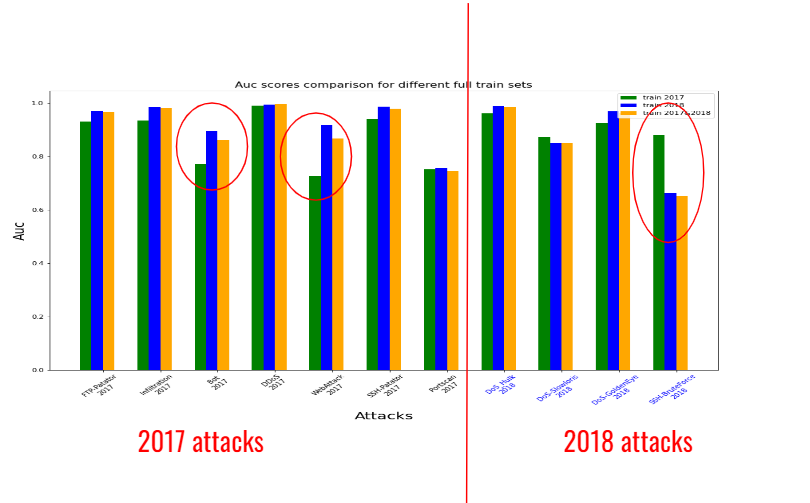
\includegraphics[width=1\linewidth]{augment.png}
    \caption{}
\end{figure}

From our experiments, we can see that using foreign datasets during training increases the AUC score. In Figure 1, when using the 2017 dataset as the test set, training with 2018 dataset or training with both 2017 and 2018 datasets outperforms training with just the 2017 dataset in most attack scenarios. Similarly, when using the 2018 dataset as the test, training with 2017 datasets or combining both datasets outperforms training with just the 2018 dataset. We have highlighted the attacks in which augmenting data with foreign datasets increased performance. As such, we conclude that, in many case, augmenting data benefits the detection system.

\begin{figure}[H]
    \centering
    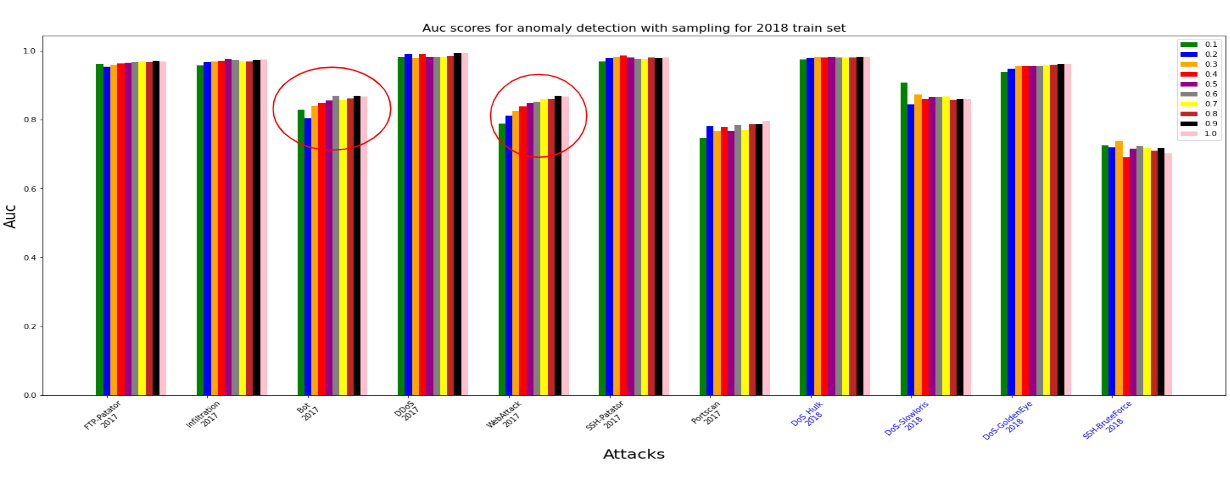
\includegraphics[width=1\linewidth]{amount.png}
    \caption{}
\end{figure}

In Figure 2, we see that only in certain attack scenarios does the amount of the data impact our result. Specifically, the BotNet 2017 and WebAttack 2017 showed strong evidence that increasing the training set size betters the AUC score. In other scenarios, we don't see a strong trend and thus the effect of dataset size on the AUC score is inconclusive.

\begin{figure}[H]
    \centering
    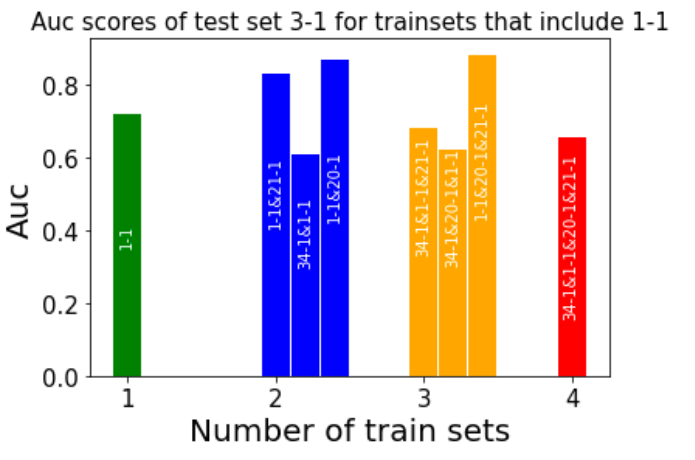
\includegraphics[width=1\linewidth]{data.png}
    \caption{}
\end{figure}

In Figure 3, we augment the data with different, foreign datasets and conclude that there is huge variance in the resulting AUC scores. This means that the type of data shared with the trainer matters as well. However, it's inconclusive exactly what type of data is the most beneficial in different attack scenarios.

\label{sec:results}

\section{Discussion}
\label{sec:discussion}

In this section, we will discuss avenues for further research.

\subsection{The many forms of diversity}

    The data we have collected seems to indicate that augmenting with shared data is more effective the further apart the individual datasets are. This makes intuitive sense: the more diverse the immune systems, the more ground they can cover and thus the less overextension the model will be forced to do. However, we are left with only a vague sense of \textit{how} diverse is optimal. (A dataset comprised exclusively of extreme points may be \textit{better} than one comprised exclusively of more central points, but it will still be inaccurate closer to the center.) Further research is required to elucidate \textbf{what protocol results in optimal data sharing.}
    
\subsection{Alternative distance functions}
    
    It is possible that AUC is not the best metric for determining what data is different enough to be useful, and that more effective diversity may be achieved using a different metric to evaluate how different the two distributions are. Thus, further research is needded to determine how the effectiveness of the model changes under different distance functions, such as mutual information, which may be closer to the ``orthogonality'' a machine learning model wants.
    
\subsection{Changes in the data to share}

    Our research thus far has focused entirely on the sharing of \textit{control} data, giving our models a more concrete picture of what normal behavior looks like in order to better spot \textit{unusual} (and thus likely to be malignant) behavior. However, it intuitively stands to reason that a model that knows some of the types of attacks it's looking for would be better at detecting those types of attack, so further research is needed to elucidate whether this is actually true -- whether sharing \textit{attack} data as well as control data may increase the effectiveness of the model.
    
\subsection{Capturing variation in the type of NIDS model}

    Our work has focused on training and refining an anomaly-based IDS model. However, the needs of a \textit{signature}-based model are different, since it needs to learn to classify specific types of attacks rather than determine where the boundary of normal and anomalous traffic lies, and it stands to reason that different techniques may be useful in training them, so further research is needed to determine how best to go about this. In addition, with high enough effectiveness it may be possible to use an anomaly-based model to help identify new signatures on which to train a signature-based model, so further research may be useful to determine the feasibility of such a technique.

\section{Conclusion}
\label{sec:conclusion}

In this paper, we evaluated the effect data sharing can have on the effectiveness of NIDS models against DDoS attacks. We suspected that, given the faults in NIDS models with SIDS having high false negative rates and AIDS’ threshold for detection being undefined, sharing extracted features from datasets of cyberattacks could help these models build an “immune system” to future attacks they may have otherwise missed. Our two main datasets, CIC-IDS and Aposemat IoT-23, were both synthetically generated for security reasons, and we processed the data to have features indicative of whether an attack occurred or not. Through out machine learning model and analysis, we found that sharing data of benign events is helpful for NIDS models and that sharing malicious data shows promise but needs further investigation. Our results indicated that the size of the training dataset may not be a large factor in the effectiveness of the model, and in many cases augmenting the data with foreign datasets may be beneficial to the detection system. There, of course, if further work to be done and ethical considerations to take into account, but we found that the process of sharing features of datasets including cyberattacks shows promise for the integrety of NIDS and network security. 


\bibliographystyle{ACM-Reference-Format}
\bibliography{reference}

\appendix

\section{Ethics}



\section{Feature Descriptions}
\label{appsec:data_description}


\end{document}
